\documentclass[a4paper,12pt]{article}
\usepackage[utf8]{inputenc}
\usepackage[italian]{babel}
\usepackage{amsfonts}
\usepackage{listings}
\usepackage{xcolor}
\usepackage{booktabs}
\usepackage{graphicx}
\usepackage{float}
\setcounter{tocdepth}{4}
\setcounter{secnumdepth}{4}

\title{Maps}
\author{Appunti di Programmazione}
\date{\today}

\begin{document}
\tableofcontents
\newpage

\maketitle

\section{Maps}

\begin{figure}[H]
    \centering
    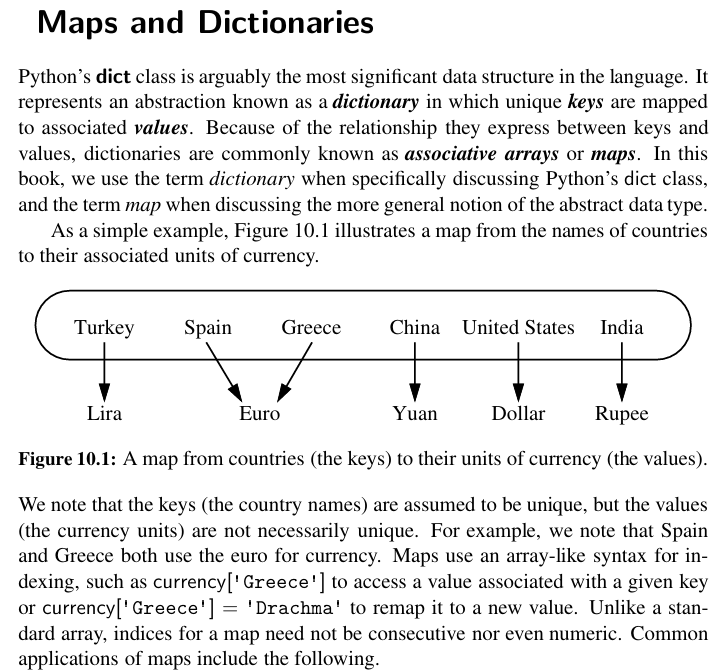
\includegraphics[width=0.7\linewidth]{Immagini/MapsDefinition.png}
    \caption{Maps definition}
\end{figure}

\subsection{Map Abstract Data Type}
Queste sono le operazioni che una Map class dovrebbe supportare:
\begin{figure}[H]
    \centering
    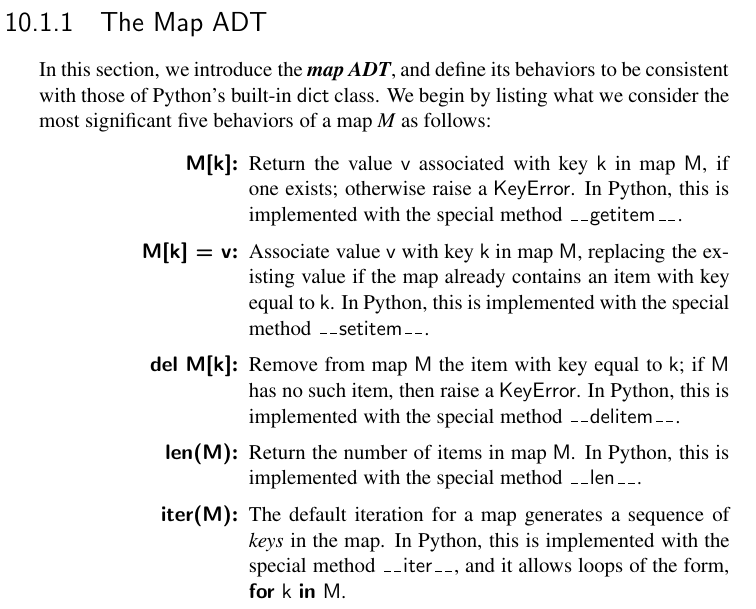
\includegraphics[width=0.48\linewidth]{Immagini/mapADT1.png}
    \vline
    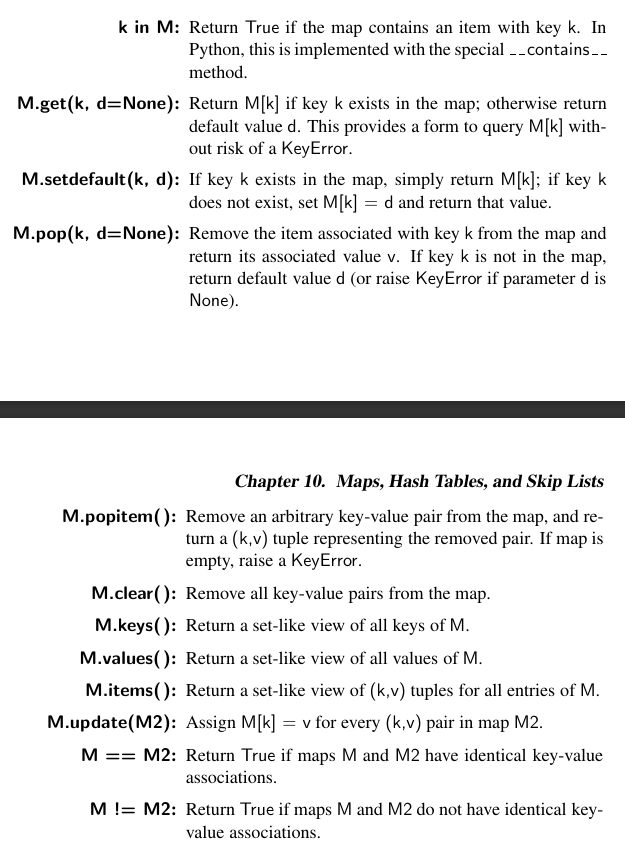
\includegraphics[width=0.48\linewidth]{Immagini/mapADT2.png}
    \caption{Map ADT}
\end{figure}

\subsubsection{Esempio di Utilizzo}

\begin{figure}[H]
    \centering
    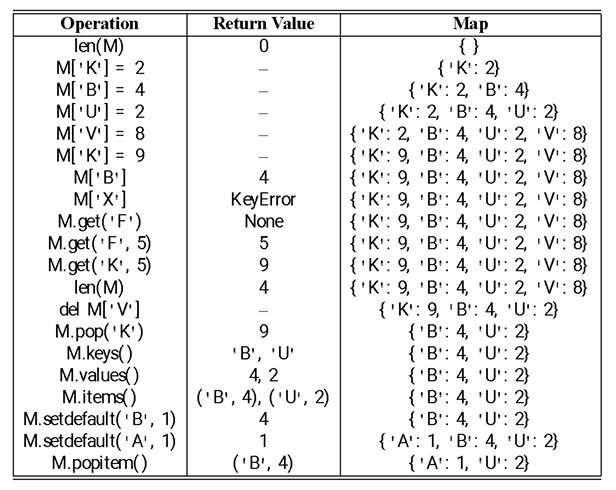
\includegraphics[width=0.7\linewidth]{Immagini/mapADT_Example.png}
    \caption{Esempio di funzionamento mapADT}
\end{figure}

\subsection{User-defined Map - Mutable Mapping ABC della Collection Module}

Per costruire le classe Maps costruiamo \textbf{MapBase} che eredità dalla Abstract Base Classe \textbf{MutableMapping}. MutableMapping è del modulo \textit{Collections}.

\begin{figure}[H]
    \centering
    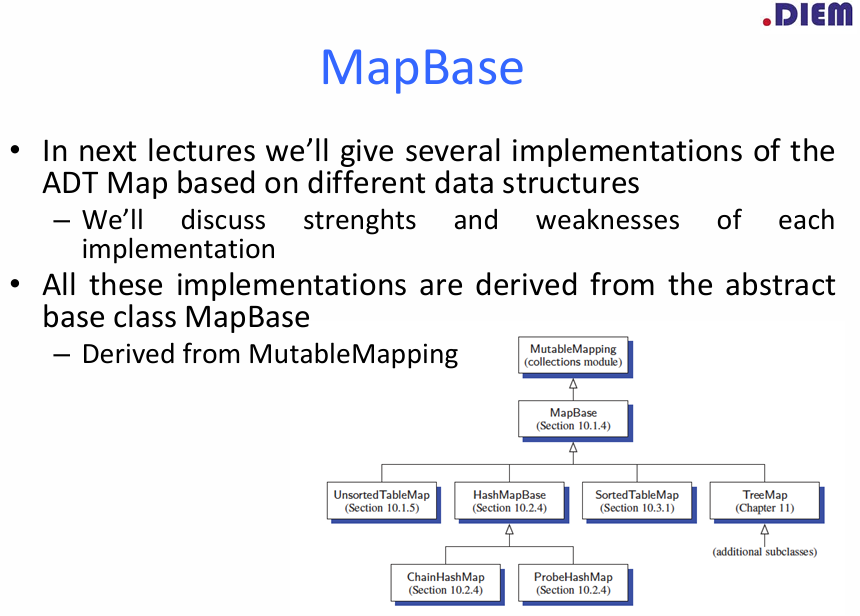
\includegraphics[width=0.47\linewidth]{Immagini/MapBase.png}
    \vline
    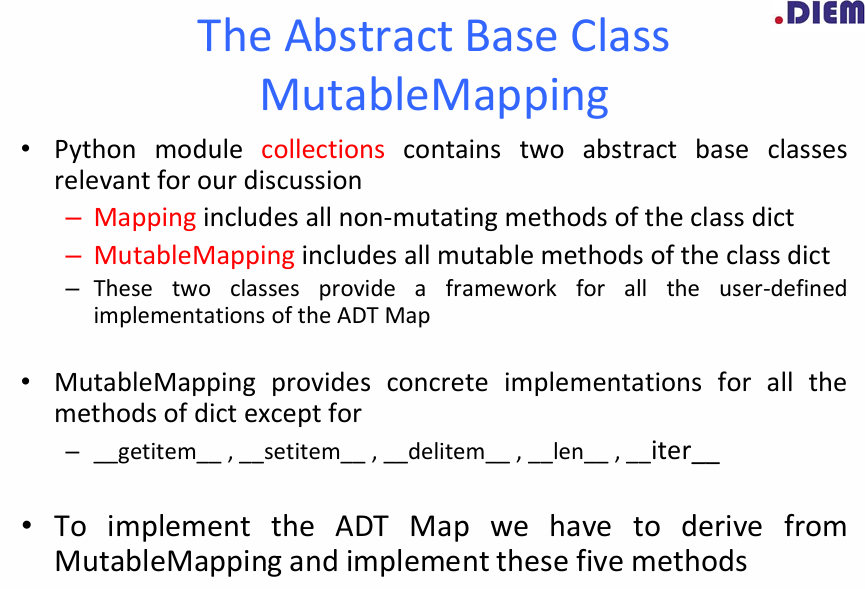
\includegraphics[width=0.47\linewidth]{Immagini/ABC_MutableMapping.png}
    \caption{Map Base e Mutable Mapping ABC}
\end{figure}

\subsection{Sorted Maps - Array Based e Binary Search Tree}
Sorted Map è una Mappa \textbf{Ordinata}, quindi è possibile definire un ordine tra le chiavi.
Sorted Map eredita da MapBase.

L'Abstract Data Type di una Sorted Map è la seguente:
\begin{figure}[H]
    \centering
    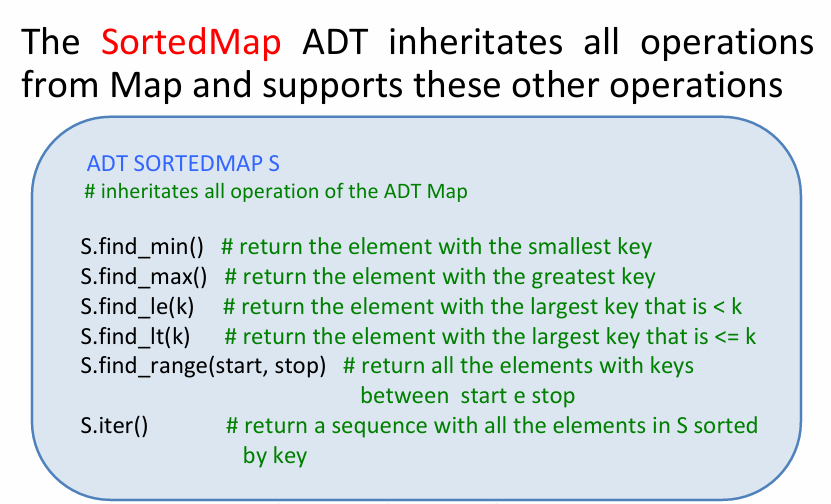
\includegraphics[width=0.7\linewidth]{Immagini/SortedMapADT.png}
    \caption{Sorted Map ADT}
\end{figure}

\subsubsection{Array Based Sorted Map}

\begin{figure}[H]
    \centering
    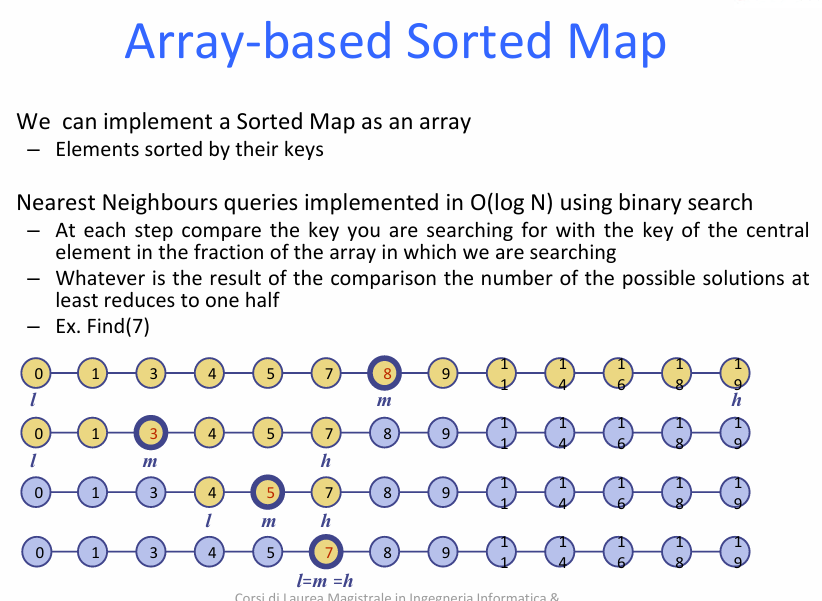
\includegraphics[width=0.47\linewidth]{Immagini/ArrayBasedSortedMap.png}
    \vline
    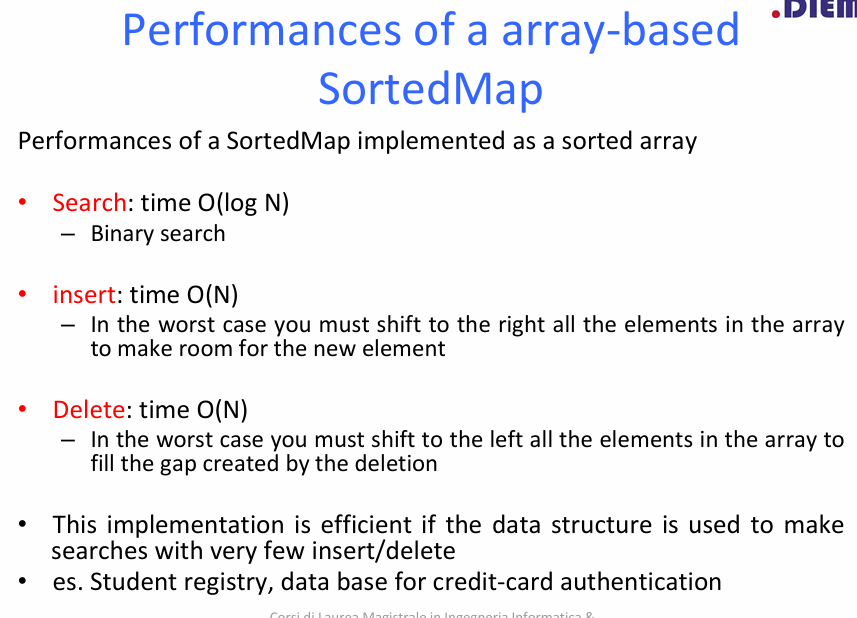
\includegraphics[width=0.47\linewidth]{Immagini/PerformanceArrayBasedSortedMap.png}
    \caption{Array Based Sorted Map}
\end{figure}

\subsubsection{Binary Search Tree Sorted Map}

\begin{figure}[H]
    \centering
    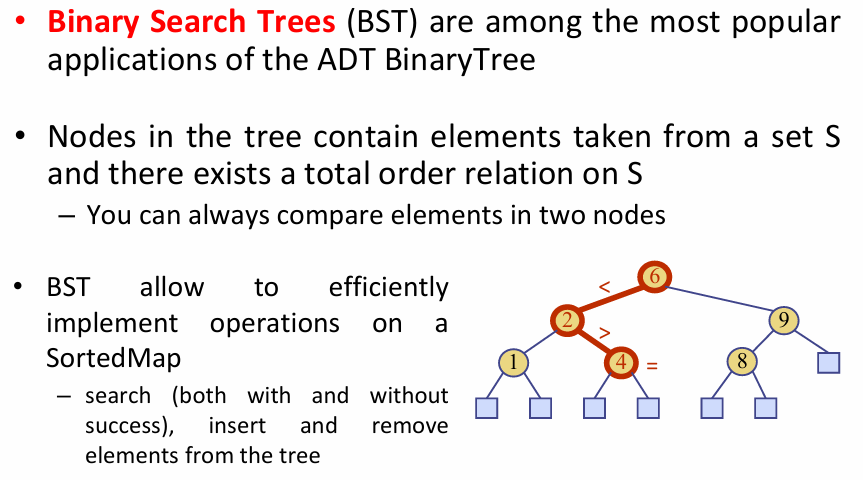
\includegraphics[width=0.47\linewidth]{Immagini/BSTSortedMap.png}
    \vline
    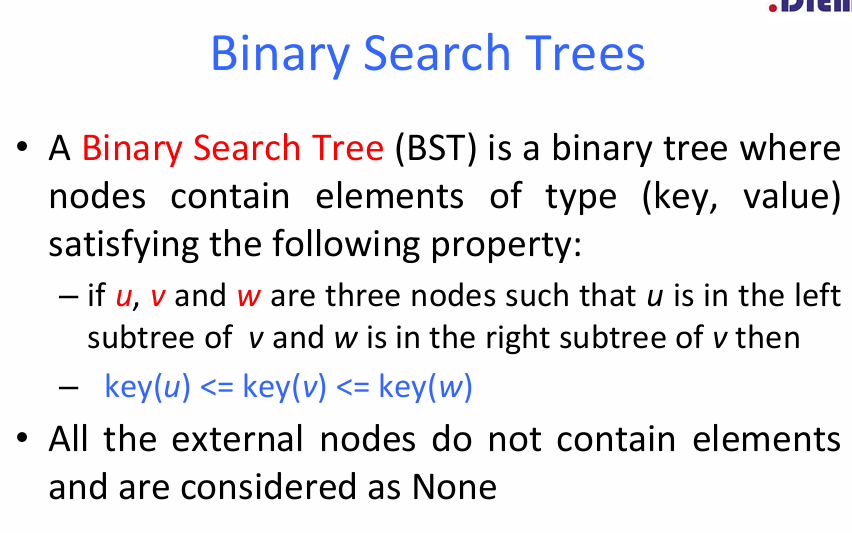
\includegraphics[width=0.47\linewidth]{Immagini/BSTDefinition.png}
    \caption{Binary Search Tree Sorted Map}
\end{figure}

\newpage
\paragraph{Predecessor \& Successor}
Pred e Succ
\begin{figure}[H]
    \centering
    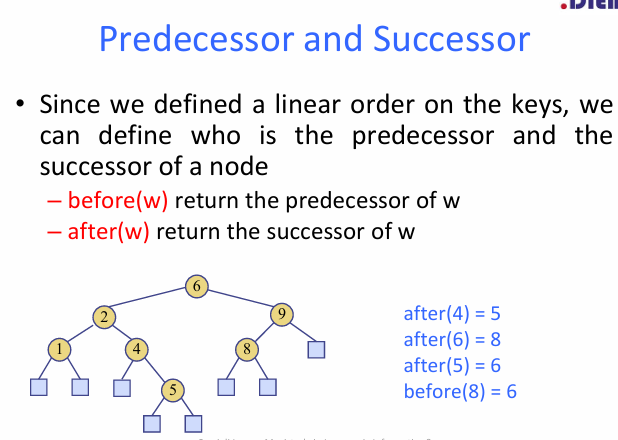
\includegraphics[width=0.47\linewidth]{Immagini/PredecessorSuccessorBST.png}
    \vline
    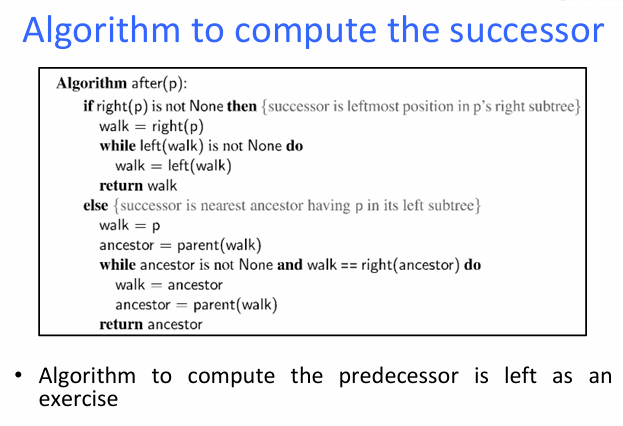
\includegraphics[width=0.47\linewidth]{Immagini/PredecessorSuccessorAlgorithm.png}
    \caption{Predecessor \& Successor}
\end{figure}

\newpage
\paragraph{Search}
Search
\begin{figure}[H]
    \centering
    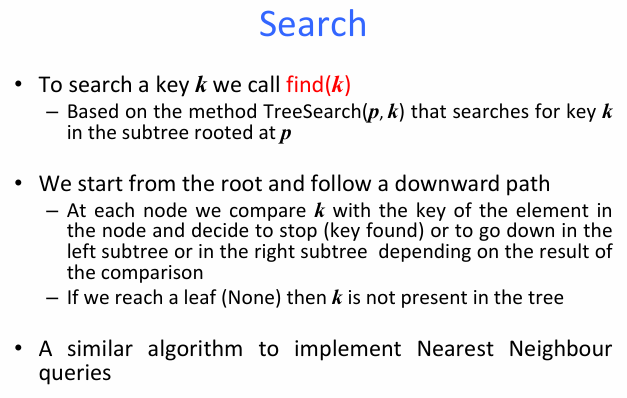
\includegraphics[width=0.47\linewidth]{Immagini/SearchBST.png}
    \vline
    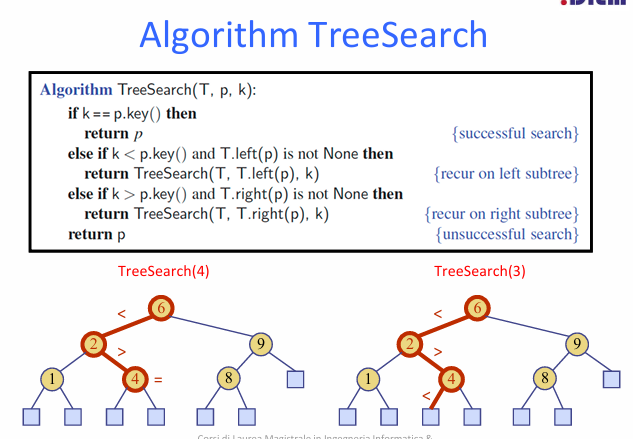
\includegraphics[width=0.47\linewidth]{Immagini/SearchBSTAlgorithm.png}
    \caption{Search}
\end{figure}

\newpage
\paragraph{Insert}
Insert
\begin{figure}[H]
    \centering
    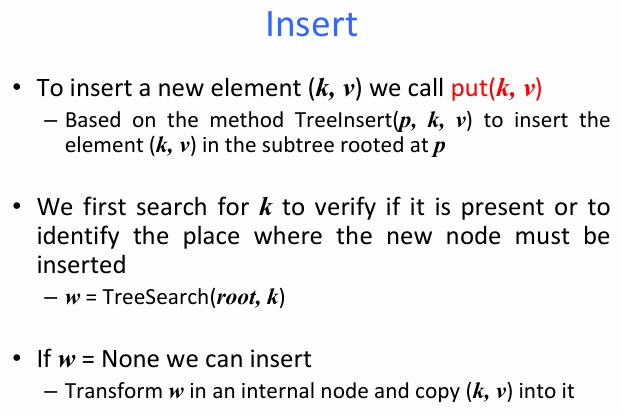
\includegraphics[width=0.47\linewidth]{Immagini/InsertBST.png}
    \vline
    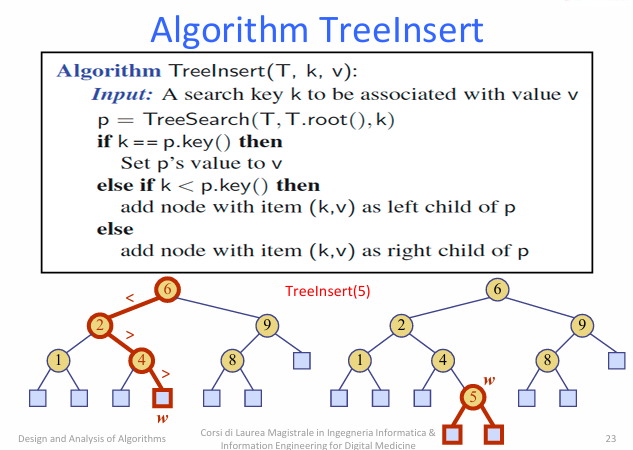
\includegraphics[width=0.47\linewidth]{Immagini/InsertBSTAlgorithm.png}
    \caption{Insert}
\end{figure}

\newpage
\paragraph{Delete}
Delete
\begin{figure}[H]
    \centering
    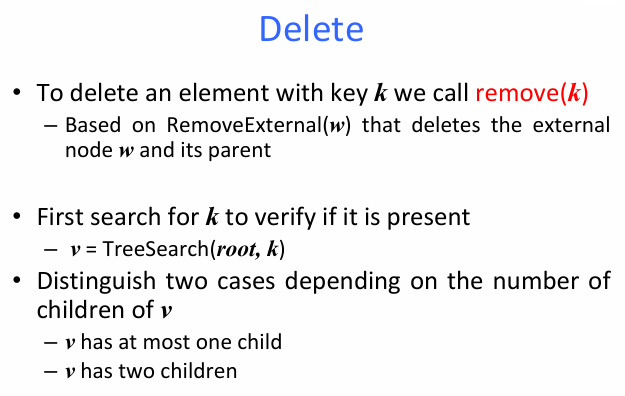
\includegraphics[width=0.47\linewidth]{Immagini/DeleteBST.png}
\end{figure}

\begin{figure}[H]
    \centering
    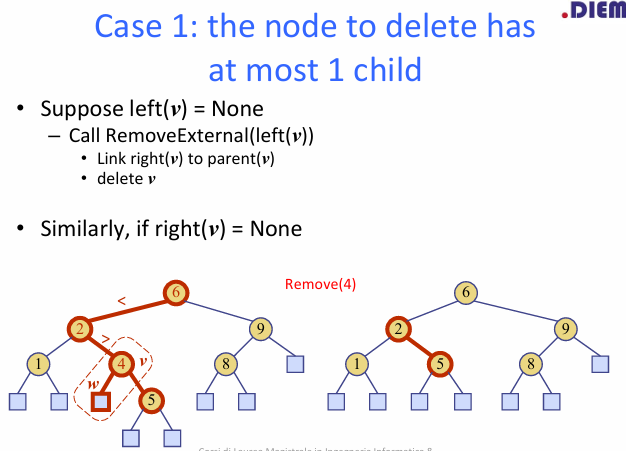
\includegraphics[width=0.47\linewidth]{Immagini/DeleteCase1.png}
    \vline
    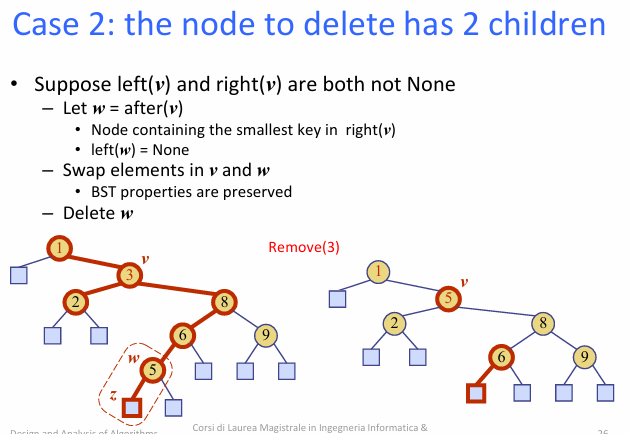
\includegraphics[width=0.47\linewidth]{Immagini/DeleteCase2.png}
    \caption{Delete}
\end{figure}

\newpage
\paragraph{Performance dei metodi PSSID }
Performances
\begin{figure}[H]
    \centering
    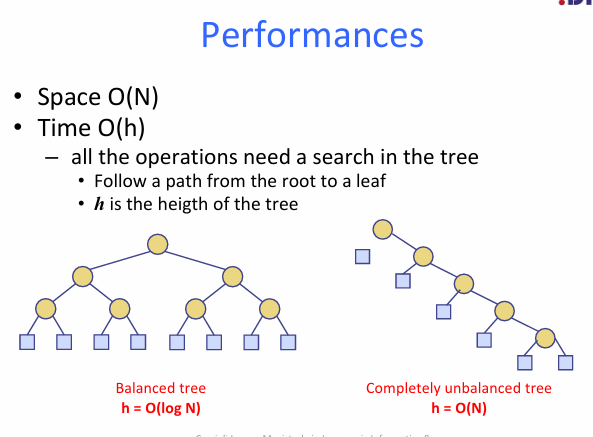
\includegraphics[width=0.47\linewidth]{Immagini/PerformanceBSTMethods.png}
    \vline
    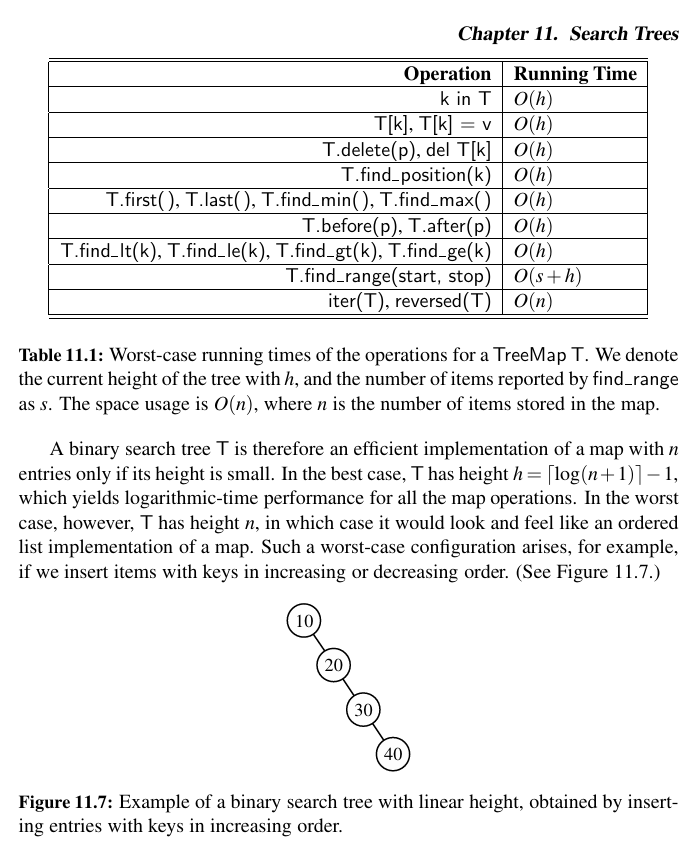
\includegraphics[width=0.47\linewidth]{Immagini/PerformancesOfBST.png}
    \caption{Performance BST Methods}
\end{figure}













\end{document}